\chapter{Dataset Exploration}
\label{chapter:dataset}

The project began with a public dataset containing metadata for over 6,800 books \cite{7k-books}. Preprocessing was necessary to enrich and validate descriptions, authorship, ratings, and structure for use in downstream models.

All transformations were performed using \texttt{pandas}, \texttt{numpy}, and visualization libraries. The pipeline was scripted in modular stages.

\section{Dataset Overview}
\label{sec:dataset-overview}

The original dataset (\texttt{books.csv}) included fields such as \texttt{isbn13}, \texttt{title}, \texttt{subtitle}, \texttt{authors}, \texttt{categories}, \texttt{description}, \texttt{published\_year}, and \texttt{average\_rating}.

Exploration focused on fields relevant to semantic search and UI rendering:

\begin{itemize}
    \item \texttt{full\_title} (from title + subtitle)
    \item \texttt{authors}
    \item \texttt{description}
    \item \texttt{average\_rating}, \texttt{published\_year}, \texttt{num\_pages}
\end{itemize}

\section{Data Cleaning and Augmentation}
\label{sec:data-cleaning}

The cleaning process included:

\begin{enumerate}
    \item Merging title and subtitle into \texttt{full\_title}
    \item Adding binary flags (e.g., \texttt{has\_description}, \texttt{has\_thumbnail})
    \item Enriching missing values from OpenLibrary (authors, years, thumbnails)
    \item Filling description gaps using the Google Books API (limited to 1,000 queries/day)
    \item Combining \texttt{subjects} and \texttt{categories} as input for classification
\end{enumerate}

Each stage included logging and result snapshots.

\section{Feature Engineering}
\label{sec:feature-engineering}

Several derived features supported later filtering:

\begin{itemize}
    \item \texttt{words\_in\_description} — Token count of final description
    \item \texttt{description\_length} — Character length of \texttt{augmented\_description}
    \item \texttt{has\_*} — Flags indicating field completeness
\end{itemize}

These helped determine which rows were usable for classification and embedding.

\section{Exploratory Analysis}
\label{sec:data-exploration}

Key visualizations were used to inform pipeline thresholds:

\begin{itemize}
    \item \textbf{Correlation heatmap:} Page count, rating, and age
    \item \textbf{Rating distribution:} Helped define UI filters
    \item \textbf{Publication histogram:} Confirmed skew toward post-2000 content
    \item \textbf{Top authors chart:} Most represented contributors
\end{itemize}

\subsection{Correlation Heatmap}
\begin{figure}[H]
    \centering
    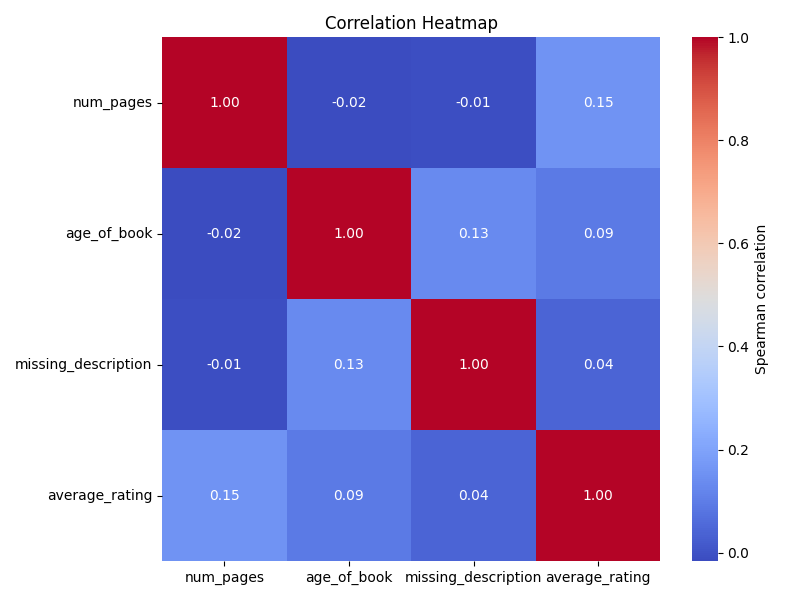
\includegraphics[width=0.7\textwidth]{figures/correlation_heatmap.png}
    \caption{Spearman Correlation Heatmap}
    \label{fig:correlation-heatmap}
\end{figure}

\subsection{Rating Distribution}
\begin{figure}[H]
    \centering
    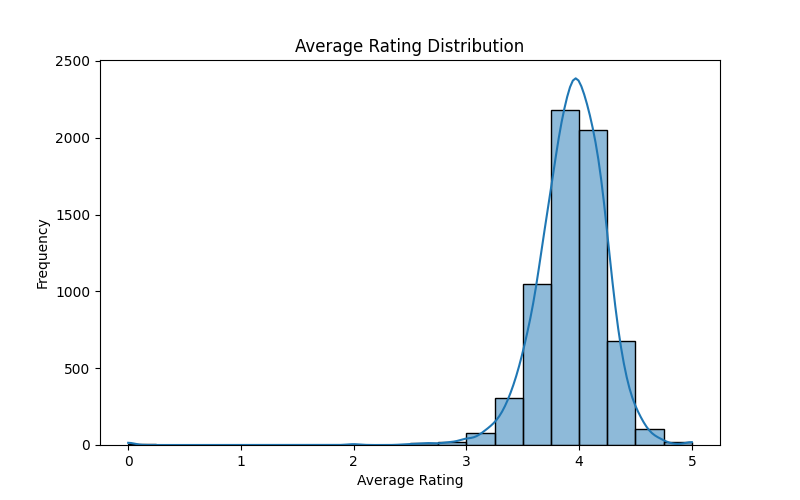
\includegraphics[width=0.7\textwidth]{figures/average_rating_distribution.png}
    \caption{Average Rating Distribution}
    \label{fig:rating-distribution}
\end{figure}

\subsection{Publication Year Distribution}
\begin{figure}[H]
    \centering
    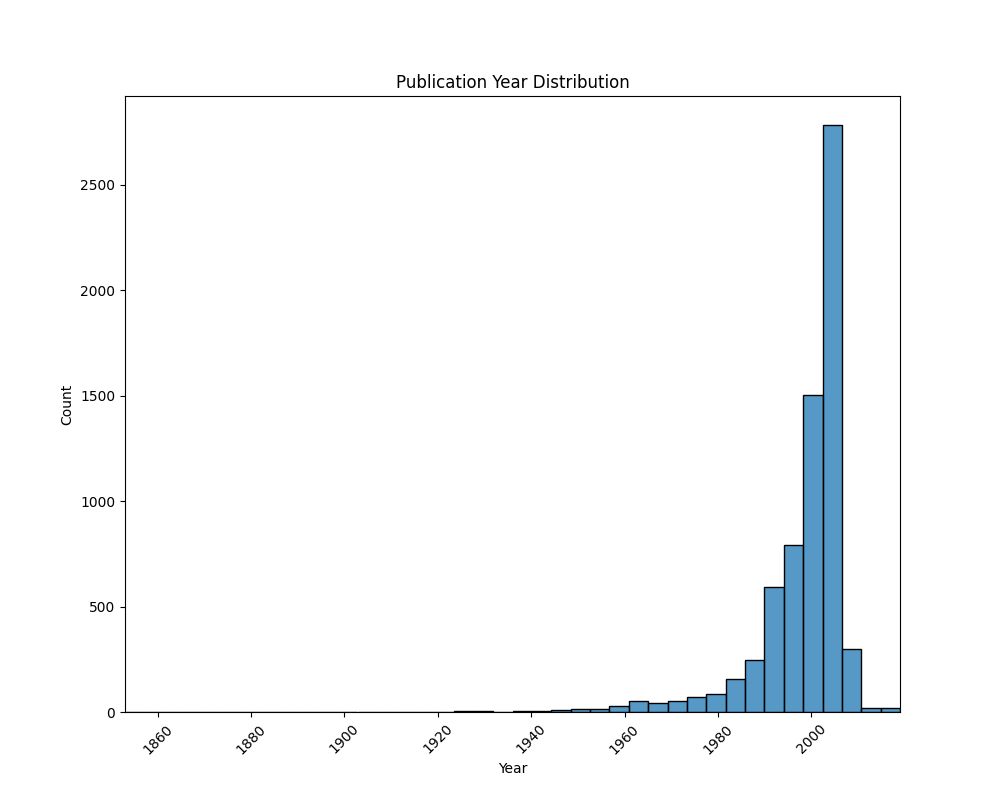
\includegraphics[width=0.7\textwidth]{figures/publication_year_distribution.png}
    \caption{Publication Year Distribution}
    \label{fig:pubyear-distribution}
\end{figure}

\subsection{Top Authors}
\label{sec:top-authors}
\begin{figure}[H]
    \centering
    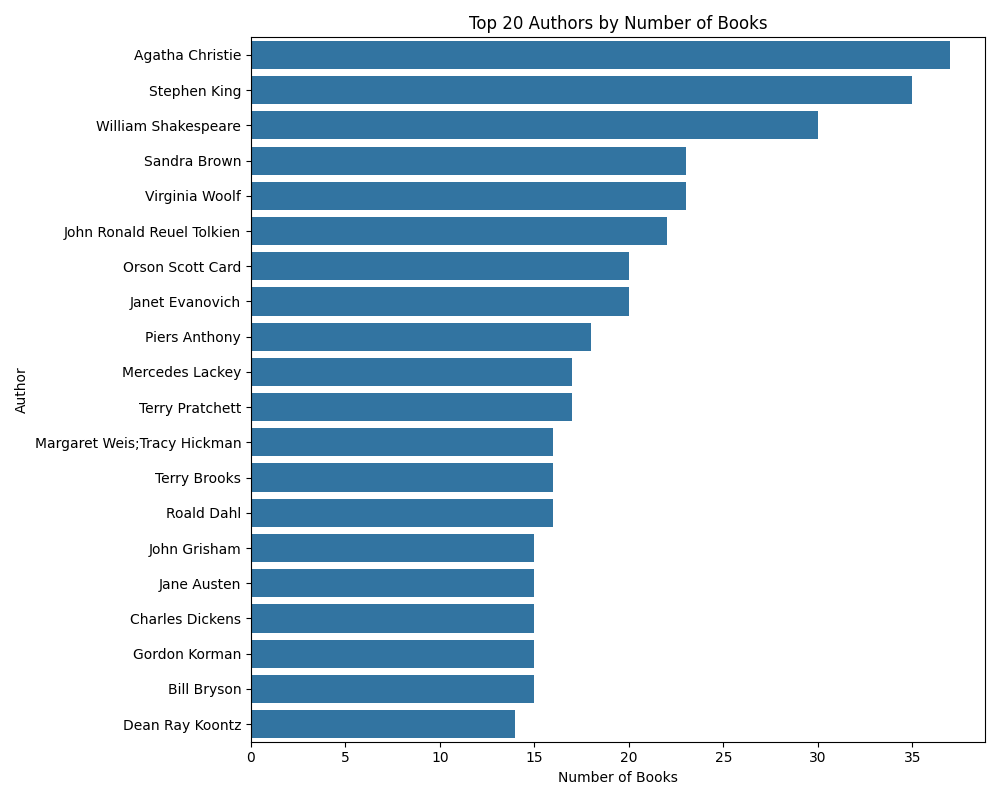
\includegraphics[width=0.8\textwidth]{figures/top_authors.png}
    \caption{Top 20 Authors by Number of Books}
    \label{fig:top-authors}
\end{figure}

\section{Outcome}
\label{sec:exploration-outcome}

Following augmentation and validation, 6,572 rows were retained. After category classification and filtering (Chapter~\ref{chapter:category-inference}), the dataset was narrowed to 5,160 well-labeled entries for embedding and indexing.
